\documentclass[slug=GL, room=HZDR\ Dresden/Rossendorf\,\ Geb.\ 620/123, supervisor=Martin\ Rehwald;\, Tim\ Ziegler]{../../Lab_Report_LaTeX/lab_report}

\title{Gaslaser}
\author{Oliver Matthes, Valentin Boettcher}
\usepackage[version=4]{mhchem}
\usepackage{todonotes}
\usepackage{amssymb}
\usepackage{graphicx,wrapfig}
\graphicspath{ {figs/} }
\newcommand{\laser}{\textsc{Laser}}
\newcommand{\hne}{\ce{HeNe}-Laser}

\newtheorem{acro}{Acronym}[section]
\begin{document}
\maketitle

\section{Einleitung}%
\label{sec:intro}
Der \laser{} ist seit seiner Erfindung in den 1960er Jahren in der
modernen Physik zu einem Standardwerkzeug geworden. Unter anderem
kann ein Laserstrahl zur Erzeugung von sehr tiefen Temperaturen
(Untersuchung von Quanteneffekten, Bose-Einstein Kondensation), zur
Erzeugung und Untersuchung von Schockwellen und zur Beschleunigung von
Elementarteilchen genutzt werden.

\todo{erlautern} Auch in der Technik findet der \laser{} aufgrund
der hohen Koh\"arenz und Intensit\"t des emmitierten Lichtstrahls
vielfach Anwendung. So hat man allt\"aglich mit auf Lasertechnologie
basierenden Barcode Scannern und CD-Spielern zu tun. Auch die moderne
Telekommunikationstechnik um das Internet nutzt \laser{} zur
Daten\"ubertragung.

Zum n\"aheren Verst\"andnis sollte zun\"achst das Akronym \laser{}
gekl\"art werden.

\begin{acro}[Laser]
\textsc{Light Amplification by Stimulated Emission of Radiation.}
\end{acro}

Dementsprechend verst\"arkt ein \laser{} also Licht durch Stimulierte
Emmision. Da die Stimulierte Emission von Strahlung ein Photon in
allen seinen Eigenschaften kopiert, wird im Allgemeinen koh\"arentes
und bedingt durch die Verst\"arkung sehr intesives Licht erzeugt.

Der grundlegende Aufbau eines Lasers ist erstaunlich einfach. So
besteht ein Laser aus:

\begin{enumerate}
\item einem aktiven Medium (Gase, Festk\"rper)
\item einem optischen Resonator (meist rotationssymmetrische, sph\"arische Spiegel)
\item einer ``Energiepumpe'' (Lichtblitze, Elektronenst\"osse)
\end{enumerate}

\begin{figure}[H]\centering
  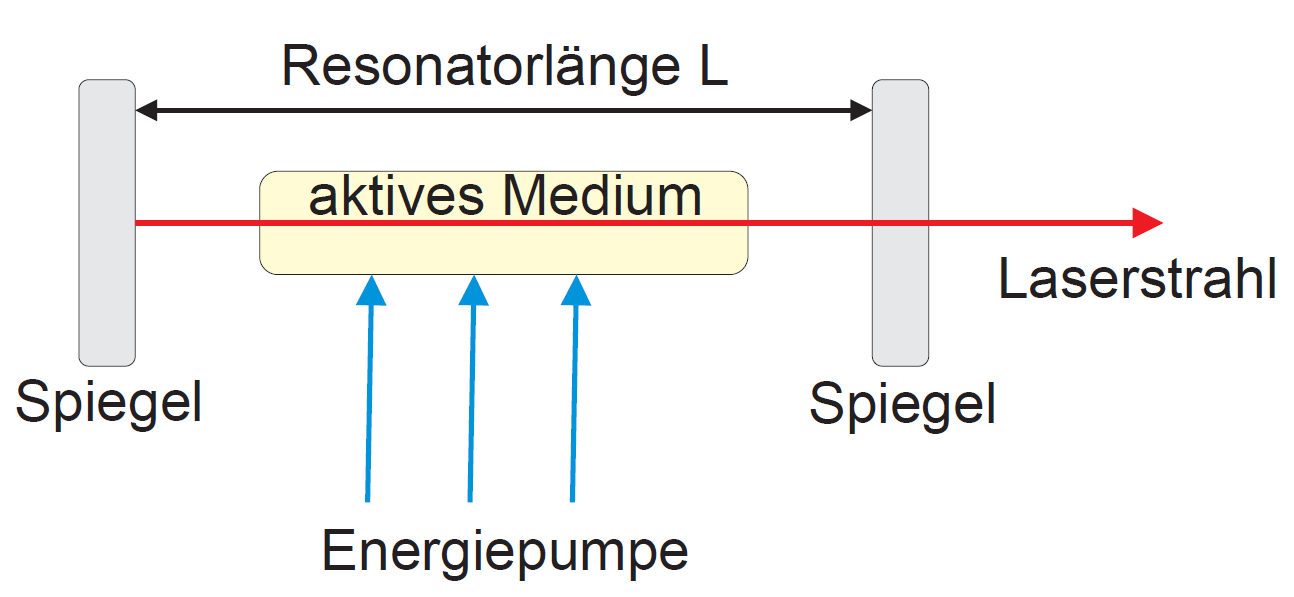
\includegraphics[width=.5\columnwidth]{schema.png}
  \caption[Aufbau]{Schema eines Lasers}
  \label{fig:aufb}
\end{figure}

Die Energiepumpe erzeugt im aktiven Medium eine
Ungleichgewichtsbesetzung von Energiniveaus, die die induzierte
Emission beg\"unstigt. Die Photonen oszillieren im Resonator mehrfach
und werden bei jedem Durchlauf verst\"arkt, bis sie den
Resonator verlassen.

\section{Theoretische Grundlagen}%
\label{sec:theo}

\subsection{Besetzungsinversion und Laserbedingung}%
\label{sec:inv}

Die Elektronen in Atomen nehmen nach der Quantenmechanik nur diskrete
Energien an. Wenn ein Elektron seinen Zustand wechselt, wird bei
diesem \"Ubergang Licht emmitiert oder absorbiert wobei f\"ur die
Energien \(E_i\) und die Frequenz des beteiligten Photons \(\nu\) gilt:

\begin{equation}
  \label{eq:transfreq}
  h\nu = E_2 - E_1
\end{equation}

Es gibt drei Prozesse, die nun die Anzahl der Atome im Grundzustand
\(N_1\) und der angeregten Atome \(N_2\) beeinflussen.

\begin{description}
\item[Absorbtion] Ein photon wird von einem Atom absorbiert, welches
  dementsprechend angeregt wird. Die H\"aufigkeit dieses Prozesses ist
  proportional zur spektralen Energiedichte.
\item[Spontane Emission] Ein angeregtes Atom geht in einen tieferen
  Zustand \"uber und sendet ein Photon aus. Dieser Prozess ist
  unabh\"angig von der umgebenden spektralen Energiedichte.
\item[Stimulierte Emission] Das Atom wird von einem passenden Photon
  zur Emmission eines zweiten, identischen Photons angeregt und geht
  in einen tieferen Zustand \"uber. Die H\"aufigkeit dieses Prozesses ist
  proportional zur spektralen Energiedichte.
\end{description}

Durch aufstellung von Ratengleichungen f\"ur das thermische
Gleichgewicht in einem Zweiniveausystem wird deutlich, dass in einem
solchen Fall die Spontane Emmission \"uberwiegt und keine
Verst\"arkung auftreten kann, da die Warscheinlichkeit f\"ur Absorbion
und Stimulierte Emmision gleich, sowie immer mehr Teilchen im
Grundzustand als im angeregten Zustand sind.

F\"ur die Photonenzahldichte \(q\) gilt mit der spektralen
Energiedichte \(\rho(\nu)\) und dem Einsteinkoeffizienten f\"ur
Stimulierte Emission und unter Vernachl\"assigung der spontanen
Emission:

\begin{equation}
  \label{eq:qrate}
  \dv{q}{t}=\rho(\nu)B_{21}(N_2-N_1)
\end{equation}

Damit eine Verst\"arkung auftritt muss gelten:

\begin{equation}
  \label{eq:first}
  \tag{Erste Laserbedingung}
  N_2>N_1
\end{equation}

Eine Besetzungsinversion kann erst mit einem Dreiniveausystem
hergestellt werden. Da dort Allerdings das untere Laserniveau der
Grundzustand ist, w\"ahre eine sehr hohe Pumprate notwendig. Bei einem
Vierniveausystem kann man durch die Nutzung eines selten thermisch
besetzten Niveaus schon mit relativ geringen Pumpraten eine
Besetzungsinversion erzeugen.

\begin{figure}[H]\centering
  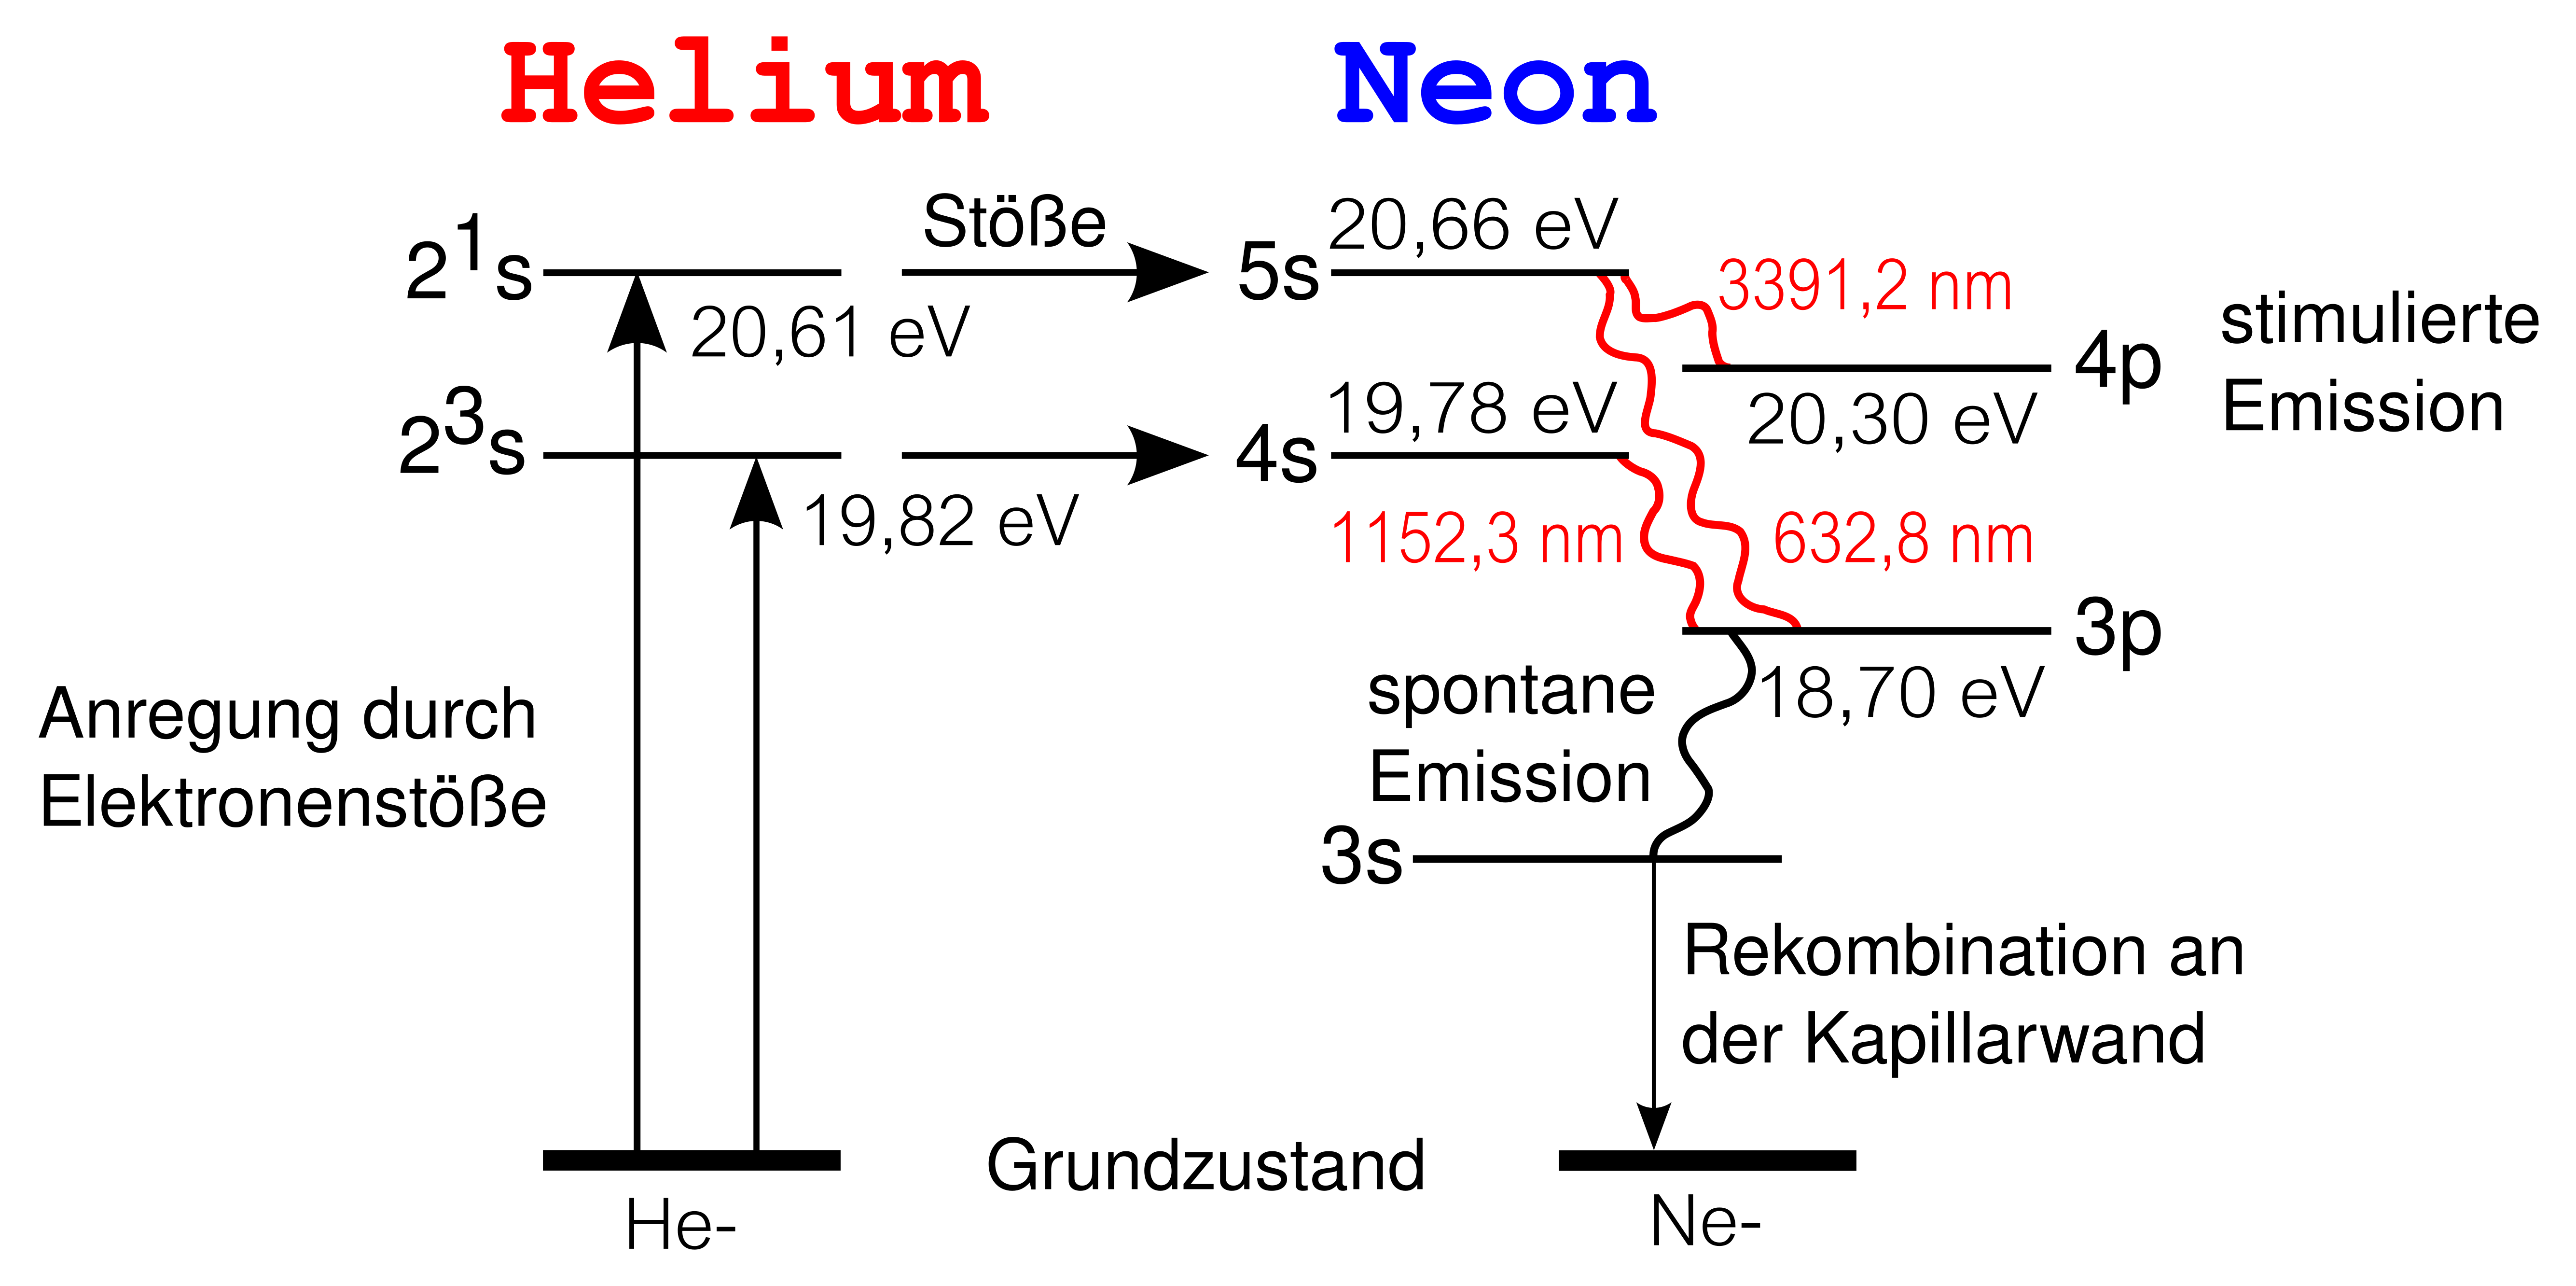
\includegraphics[width=.8\columnwidth]{heneniv.png}
  \caption[Aufbau]{Vierniveausystem des \hne{}}
  \label{fig:niveaus}
\end{figure}

Der \hne{} basiert auf dem in~\ref{fig:niveaus} dargestellten
Vierniveausystem. Das Helium wird (z.B. mit Elektronenst\"o\ss{}en)
angeregt (nach \(2^1S\) bzw. \(2^3S\)) und \"ubertr\"agt diese
Anregungung durch Atomst\"o\ss{}e an das Neon, dessen Niveaus (\(5S\),
\(4S\)) \"ahnlich liegen. Der im optisch sichtbaren Bereich liegende
\"Ubergang \(5S\rightarrow 3P\) wird vorwiegend im \hne{} genutzt und
ist f\"ur eine Besetzungsinversion besonders vorteilhaft, da die
Lebensdauer der \(S\) Niveaus h\"oher als die der \(P\) Niveaus ist.


Um nun die Verst\"arkungswirkung des Lasers in Anwendungen zu nutzen,
ist eine Betrachtung von Energieverlusten n\"otig. \"Ublicherweise
durchqueren Photonen einen Resonator der L\"ange \(L\) mehrfach und
werden dabei durch stimulierte Emission verst\"arkt. Allerdings treten
auch immer Verluste auf, sodass sich pro doppelten Umlauf die
Intensit\"at um einen Faktor \(e^{-\kappa}\) korrigiert werden muss,
wobei \(\kappa\) der sog. Verlustkoeffizient ist. Nach dieser
Betrachtung muss die Verst\"arkung gr\"o\ss{}er sein als der Verlust.
Mit dem Wirkungsquerschnitt \(\sigma_{21}=B_{21}\frac{h\cdot\nu}{c}\)
ergibt sich:

\begin{equation}
  \label{eq:zwlabe}
  \tag{zweite Laserbedingung}
  \sigma_{21}(N_2-N_1)\cdot 2L \geq \kappa
\end{equation}

Falls nur Verluste bei der Reflexion an den Resonatorspiegeln
auftreten, gilt mit den Reflexionskoeffizienten \(r_1,r_2\):

\begin{equation}
  \label{eq:kappa}
  \kappa = - \ln(r_1\cdot r_2)
\end{equation}

Falls der Laserprozess stabil ist, stellt sich ein Gleichgewicht ein
und die \ref{eq:zwlabe} gilt mit einem Gleichheitszeichen.

\subsection{Optischer Resonator}
\label{sec:reso}

Ein optischer Resonator besteht im einfachsten Fall aus zwei Spiegeln
mit den Radien \(R_1,R_2\) im Abstand \(L\). (Siehe auch
\ref{fig:aufb}.)

% Damit ein Stabiler Lasing prozess m\"oglich ist, muss sich ein
% station\"ares Wellenfeld ausbilden.
Damit sich in longitudinaler Richtung eine stehende Welle ausbilden
kann, muss L ein Vielfaches der halben Wellenl\"ange des Lichtes sein.
Der Abstand der m\"oglichen Frequenzen (Moden) betr\"agt daher:

\begin{equation}
  \label{eq:longmodes}
  \Delta\nu = \frac{c}{2L}
\end{equation}

Wenn man die elektromagnetische Wellengleichung f\"ur in der
\(x,y\)-Ebene langsam ver\"anderliche Felder n\"ahert (paraxial)
ergeben sich analytische L\"osungen f\"uhr strahlenartige Felder.
Diese Strahlen zeigen in transversaler Richtung unterschiedliche
Intesit\"atsverteilungen von denen die einfachste und am wenigsten
divergierende Mode die Form einer Gaussverteilung hat:
\textbf{Gau\ss{}-Strahl}

\begin{figure}[H]\centering
  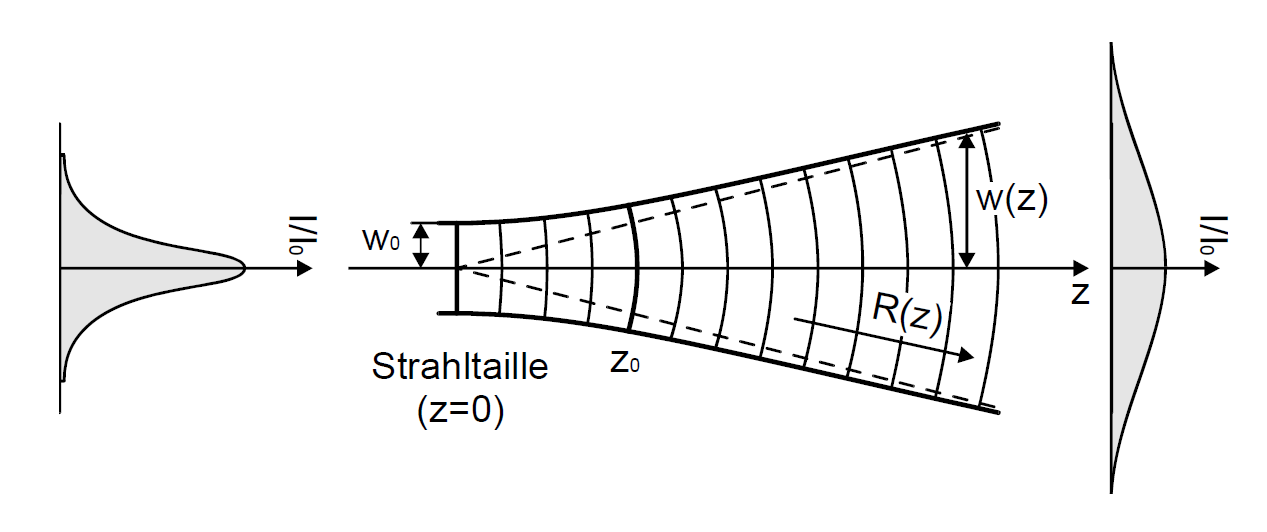
\includegraphics[width=.5\columnwidth]{gauss-strahl.png}
  \caption[Gauss]{Gau\ss{}-Strahl }
  \label{fig:gauss}
\end{figure}

Dieser Strahl wird, wie in~\ref{fig:gauss} ersichtlich, charakterisiert durch
die Strahldicke \(w(z)\) und den Radius der Wellenfronten
\(R(z)\). Die Angabe von Amplitude, Strahltaille \(w(z=0)=w_0\) und
Wellenl\"ange beschreibt den Strahl vollst\"andig.

\subsubsection{Matrizenopik}
\label{sec:matrizen}

Um eine Stabilit\"atsbedingung f\"ur den Resonator aufzustellen, muss
zuerst das Verhalten des Lichtfeldes beschrieben werden. Die
Matrizenmethode der Strahlenoptik ist auch auf Gau\ss{}strahlen
anwendbar und stellt daher ein probates Mittel dar. Diese Basiert auf
der zweidimensionalen Darstellung des Lichtstrahles durch einen
Vektor:

\begin{equation}
  \mqty(d \\ \alpha) \widehat{=} \mqty(\text{Abstand zur Achse} \\
  \text{Winkel zur Achse})
\end{equation}

Das optische System wird durch eine Matrix dargestellt, die man
eleganterweise durch multiplikation der Matrizen der einzelsysteme
erh\"alt.

\begin{equation}
  \label{eq:systmatrix}
  \mathfrak{M}_{\text{System}}=\mathfrak{M}_{\text{1}}\cdot\ldots\cdot\mathfrak{M}_{n}=\mqty(A
  & B \\ C & D)
\end{equation}

Die hier ben\"otigten Matrizen sind im folgenden aufgef\"uhrt.
{\setlength{\tabcolsep}{20pt}
\begin{table}[h!]
  \centering
  \begin{tabular}{l | c | l}
    \textbf{Element} & \textbf{Matrix} & \textbf{Parameter} \\
    \midrule\\
    \addlinespace[-2ex]
    freie Ausbreitung & \(\begin{pmatrix}
      1 & s \\
      0 & 1
    \end{pmatrix}\) & Wegl\"ange \(s\) \\
    \midrule\\
    \addlinespace[-2ex]
    d\"unne Linse & \(\begin{pmatrix}
      1 & 0 \\
      -1/f & 1
    \end{pmatrix}\) & Brennweite \(f\) \\
    \midrule\\
    \addlinespace[-2ex]
    sph\"arischer Spiegel & \(\begin{pmatrix}
      1 & 0 \\
      -2/R & 1
    \end{pmatrix}\) & Radius \(R\) \\

  \end{tabular}
  \caption{Einige optische Matrizen}
  \label{tab:mats}
\end{table}}

Definiert man \(\frac{1}{q(z)}=\frac{1}{R(z)}+i\frac{\lambda}{\pi
  w^2(z)}=a+i\cdot b\) so transformiert sich dieser Parameter mit der Matrix
\(\mathfrak{M}_{\text{System}}\) wie folgt:

\begin{equation}
  \label{eq:qtrans}
  q'=\frac{Aq + B}{Cq+D}
\end{equation}

So kann man die Kaustik eines Laserstrahls, der in einem
Hemisph\"arischen Resonator entsteht und durch eine Linse mit
Brennweite \(f\) fokussiert wie folgt berechnet.

Da \(R_2=\infty\) kann man \(z=0\) (postition des Beamwaist) auf die
Spiegelposition legen.  Aus dem in~\ref{sec:stabres} diskutierten
Anpassungen, ergibt sich der Beamwaist am Endspiegel zu:

\begin{equation}
  \label{eq:konfwaist}
  w_0^4=\qty(\frac{\lambda}{\pi})^2L(R-L)
\end{equation}

Wenn \(s\) den Weg vor der Linse und \(x\) den Weg nach der Linse
bezeichnet, dann ergibt sich f\"ur den Imagin\"arteil von \(q'\):

\begin{equation}
  \label{eq:qkaust}
  b'=b\cdot\frac{AD-CB}{A^2+B^2b^2}
\end{equation}

Damit kann man den Beamwaist des resultierenden Strahls berechen:

\begin{equation}
  \label{eq:reswaist}
  w'=\sqrt{\frac{\lambda}{\pi\cdot b'(x)}}
\end{equation}


\subsubsection{Stabilit\"at im Resonator}
\label{sec:stabres}

Wenn man den Gau\ss{}strahl so anpasst, dass \(R(z_1)=R_1,\;
R(z_2)=R_2\) (siehe \ref{fig:gauss-res}) und fordert, dass der Strahl
nach zweifacher Reflexion in sich selbst \"ubergeht, so kann man ein
geometrisches Kriterium f\"ur die Resonatorstabilit\"at.

\begin{wrapfigure}{r}{10cm}
  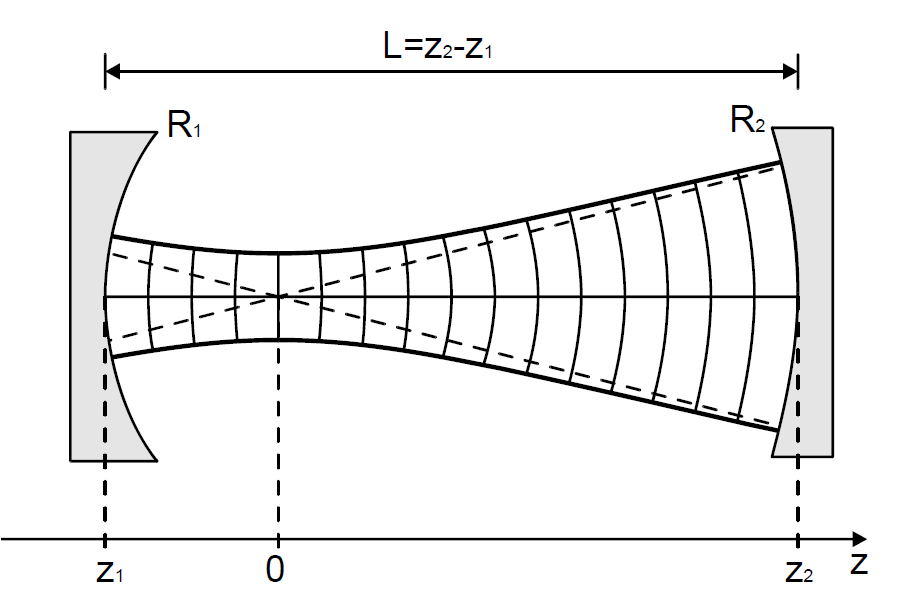
\includegraphics[width=10cm]{gauss-res.png}
  \caption[Gauss]{Gau\ss{}-Strahl im Resonator}
  \label{fig:gauss-res}
\end{wrapfigure}

Mit der Defintion
\begin{equation}
  \label{eq:gparams}
  g_i=1-\frac{L}{R_i};\; i=1,2
\end{equation}

ist ein Resonator stabil, falls:
\begin{equation}
  \label{eq:stabbed}
  0\leq g_1g_2\leq 1
\end{equation}

\subsection{Modenstruktur und Linienverbreiterung des Laser-Lichtes}
\label{ref:linv}

Da, wie in~\ref{sec:reso} diskutiert, mehrere Moden im Resonator
stabil sind, werden im Allgemeinen auch mehrere Moden verst\"arkt.
Unterschiedliche Moden werden in der Regel unterschiedlich
verst\"arkt, sodass nur endlich viele Moden die~\ref{eq:zwlabe}
erf\"ullen, also \"uber der Verlustgrenze liegen.

Das h\"ohere transversale Moden schneller Divergieren als die
Gau\ss{}mode, sind bei diesen Moden die Beugungsverluste gr\"o\ss{}er,
sodass meist nur wenige davon \"uber der Verlustgrenze liegen. \todo{quelle!}

Die Longitudinalen Moden unterscheiden sich in ihren Frequenzen und
liegen mit steigender Resonatorl\"ange zunehmend dicht
(\ref{eq:longmodes}). Die stimulierte Emission akzeptiert aufgrund der
sog. \textbf{Linienverbreiterung} mehrere Frequenzen, also mehrere
longitudinale Moden, die sich die Besetzungsinversion teilen m\"ussen.

F\"ur die Linienverbreiterung sind unter anderem die Energie-Zeit
Unsch\"arfe, strahlungsfreie \"Uberg\"ange, elastische St\"o\ss{}e
(Druckverbreiterung) und der Dopplereffekt (Dopplerverbreiterung)
verantwortlich. Dabei unterscheidet zwischen \textit{homogener-} (die
ersten drei Beispiele) und \textit{inhomogener} Linienverbreiterung,
wobei erstere auf alle Gasatome gleichzeitig und letztere nur auf
bestimmte Atomgruppen wirkt. \todo{ev. folgen, quelle!}

Beim \hne{} in diesem Versuch \"uberwiegt die Dopplerverbreitung,
deren halbwertsbreite hier angegeben werden soll.

\begin{equation}
  \label{eq:doppler}
  (\Delta\nu)_{\text{Doppler}}=2\cdot \nu_0\qty(\frac{2kT\ln{2}}{mc^2})^{1/2}
\end{equation}

\begin{conditions}
  T & Temperatur \\
  \nu_0 & Zentralfrequenz \\
  m & mittlere Atommasse
\end{conditions}
\todo{Brewsterfenster}

\subsection{Fabry-Perot-Interferometer}
\label{sec:fabry}

Das \textit{Fabry-Perot-Interferometer} (im Folgenden FPI) beruht auf
Vielstrahlinterferenz, worin sich auch seine hohe spektrale
Aufl\"osung begr\"undet. Die einfallende Welle wird zwischen zwei
planparallelen Fl\"achen (genannt Etalon, Abstand \(d\),
Reflexionsverm\"ogen \(R\)) sehr oft reflektiert. Die Wellen, die das
Etalon verlassen, interferieren nur bei bestimmten Abst\"anden \(d\)
oder Wellenl\"angen \(\lambda\) konstruktiv.

Damit kann das FPI sowohl als Interferometer zur Messung von
Frequenzen, als auch als Modenfilter eingesetzt werden.

Der \textit{freie Spektralbereich} (FSR) des FPI gibt an, wie weit die
Einzelnen passierenden Frequenzen auseinander liegen und kann zur
Kalibrierung von Frequenzdifferenzen genutzt werden.
Es gilt:

\begin{equation}
  \label{eq:fsr}
  \text{FSR} = \frac{c}{2\cdot d} = \delta\nu
\end{equation}

Die \textit{Finesse} des FPI ist der Quotien aus FSR und
Halbwertsbreite der Peaks, also ein Ma\ss{} f\"ur die Aufl\"osung des
FPI:

\begin{equation}
  \label{eq:finesse}
  \mathfrak{F} = \frac{\pi\sqrt{R}}{1-R}
\end{equation}

Es sollte also \(R\rightarrow 1\) gelten.

Es ist zu beachten, dass die hier aufgef\"uhrten Beziehungen nur bei
senkrechten Strahleinfall gelten.

\subsection{Malus Law}
\label{sec:malus}

Die Intensit\"at einer Ebenen Welle nach einem Polfilter ergibt sich
durch Projektion der Eingangswelle auf die Richtung des Filters. Die
Quadratur ergibt sich aus der Intensit\"atsberechnung \(\propto
E^2\). \(\Theta\) bezeichnet den relativen Winkel der
Polarisationsrichtungen.

\begin{equation}
  \label{eq:malus}
  I(\Theta)=I_0\cdot \cos^2{\Theta}
\end{equation}

\section{Versuchaufbau und Ger\"ate}
\label{sec:versuaufb}

Der Versuchaufbau ist schematisch in~\ref{fig:aufb} dargestellt und umfasst unter anderem:

\begin{description}
\item[Spiegel] Nummeriert von 1 bis 10.
\item[Laser] Kommerzieller \hne{} und gr\"uner Justagelaser.
\item[Blenden] Als Justagehilfe und zum Ausblenden von unerw\"unschten Moden.
\item[Linsen und Filter] Zur Untersuchung der Strahleigenschaften. (Sammellinse, Polfilter, Graufilter)
\item[Fabry Perot Interferometer] Festaufbau, Konfokal
\item[Leistungsmessger\"at] Zur Leistungsmessung und als Justagehilfe.
\item[Faserspektrometer] \textsc{Ocean Optics HR2000+} als Referenzmessger\"at.
\end{description}


\begin{figure}[H]\centering
  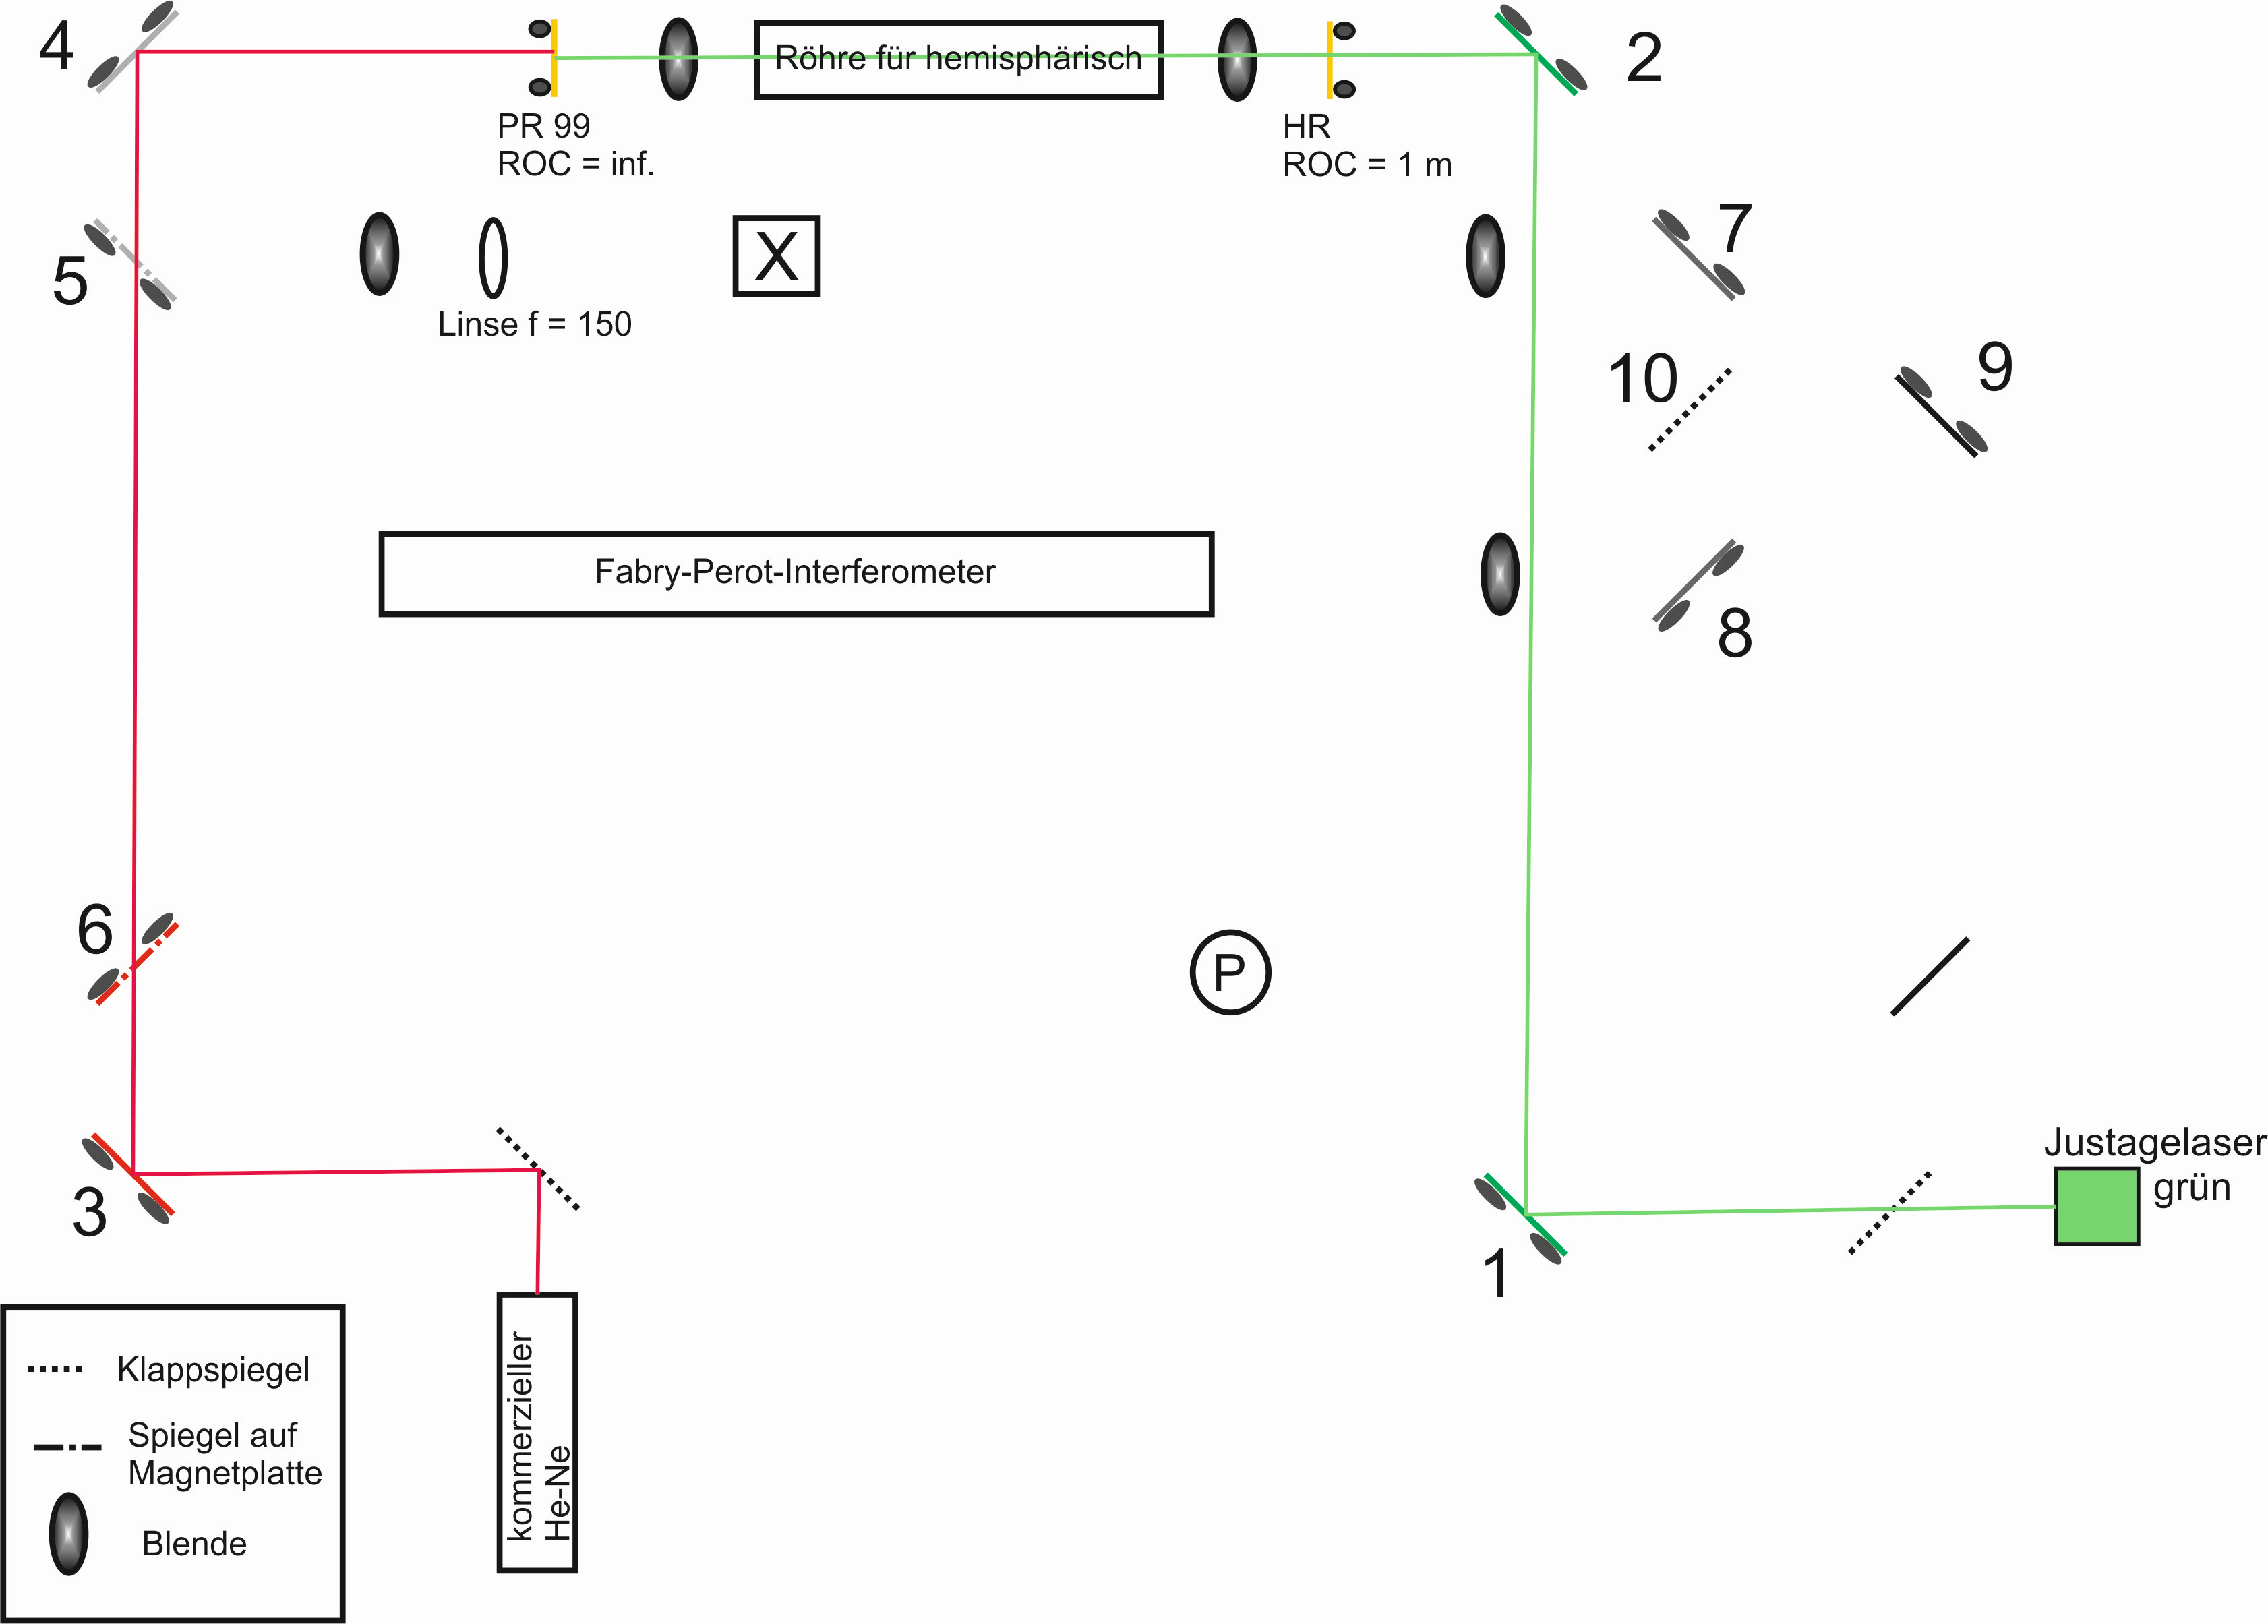
\includegraphics[width=.5\columnwidth]{aufb.png}
  \caption[Aufbau]{Versuchsaufbau}
  \label{fig:aufb}
\end{figure}



\section{Durchf\"uhrung}
\label{sec:durch}

\subsection{Stabilit\"atsbereich}
\label{sec:stabber}

Da \(g_1(R_1=\infty)=1\) folgt mit \(R_2=\SI{1}{\meter}\) und \(0\leq g_2\leq 1\):

\begin{equation}
  \label{eq:stabber}
  \SI{0}{\meter}\leq L \leq \SI{1}{\meter}
\end{equation}

Das ist auch aus dem Stabilit\"atsdiagramm ersichtlich.
\begin{figure}[H]\centering
  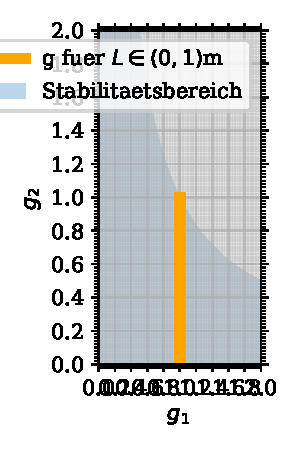
\includegraphics[width=.5\columnwidth]{figs/stabdiag.pdf}
  \caption[Gauss]{Stabilit\"atsdiagramm}
  \label{fig:stabdiag}
\end{figure}

\subsection{Justage und Messung der Verst\"arkung im Einfachdurchgang}
\label{sec:justage}

Durch Anpassen der Spiegel 4 und 5 und zweier Blenden auf der
Optischen Achse (OA) der \ce{HeNe}-R\"ohre wurde der Rote Laser
parallel zur OA ausgerichtet, sodass er die R\"ohre ohne st\"orende
Reflexe an den Kappilarw\"anden passierte. Auf \"ahnliche Weise
geschah das auch mit dem gr\"unen Laser (\"uber Spiegel 1, 2).

Anschlie\ss{}end wurde die Leistung des kommerziellen Lasers vor der
R\"ohre und bei Durchgang durch diese im deaktivierten und im aktiven
Zustand, sowie der Untergrund de Powermeters gemessen. Bei allen
Leistungsmessungen wurde die Raumbeleuchtung abgeschaltet. Die
Messzeit wurde auf \SI{150}{\second} festgelegt, da die Schwankung
des Messwertes ab dieser Zeit ann\"hernd konstant blieb.

\subsection{Aufbau des Hemisph\"arischen Resonators}
\label{sec:aufbauhemi}

Nach dem Einbau der Resonatorspiegel wurde deren Justage mit Hilfe von
R\"uckreflexen der Justagelaser durchgef\"uhrt. Die anf\"angliche
Leistung des Lasers war gering, konnte jedoch durch Beamwalken
erheblich gesteigert werden (auf ca \SI{1}{\milli\watt}).

Anschlie\ss{}end wurde der Laserstrahl auf eine zweite optische Bahn
justiert und die Ausgangsleistung des Lasers in Abeh\"angigkeit der
Resonatorl\"ange gemessen. Die L\"ange wurde durch Verschieben des
gekr\"ummten Spiegels verstellt.

\subsection{Messung der Polarisationseigenschafte}
\label{sec:poleig}

Nach Einstellung der Resonatorl\"ange auf \SI{80}{\centi\meter}, wurde
ein Polarisationsfilter in den Strahlengang gebracht und die
transmittierte Leistung in Abh\"angigkeit des Polfilterwinkels
gemessen.
Die Messzeit wurde aus Zeitgr\"unden auf \SI{1}{\minute} reduziert.
Da die Polarisationsrichtung des Lasers mit der Nullstellung des
Polfilters \"ubereinstimmte, konnte der Polarisationswinkel absolut
abgelesen werden.

\section{Auswertung}
\label{sec:auswertung}

\subsection{Verst\"arkung im Einfachdurchgang}
\label{sec:ausweinf}

\begin{table}[h]
  \begin{tabular}{l|SSSS}
    \toprule
    & {Mittelwert [\si{\micro\watt}]} & {Standartabweichung
                                      [\si{\micro\watt}]} & {Minimum
                                                            [\si{\micro\watt}]}
    & {Maximum [\si{\micro\watt}]} \\
    \midrule
    Untergrund & 0.839 & 0.031 & 0.771 & 0.888 \\
    R\"ohre aktiv & 965.161  & 4.2  & 958.229  & 973.112  \\
    R\"ohre inaktiv & 907.161  & 17.5 & 885.229  & 949.112  \\
    vor R\"ohre & 1319.161 & 2.0  & 1319.229 & 1329.112 \\
    \bottomrule
  \end{tabular}
  \caption{Leistungsmessungen des Einfachdurchgangs mit abgezogenem Untergrund}
  \label{tab:leistungeinfach}
\end{table}

Die Systematischen Messungenaugkeiten liegen beim Powermeter weit
unter der statistischen Schwankung und werden hier vernachl\"assigt.

Der untergrund der Messung ist in Relation zum Rest der Messungen
relativ gering und wurde in~\ref{tab:leistungeinfach} abgezogen. Da
er jedoch eine gr\"o\ss{}ordnung unter den \"ublichen Messwerten und
deren statistischer Schwankung liegt, wird der Untergrund in allen
folgenden Messungen vernachl\"assigt, weil Messbereiche nicht
vergleichbar sind.
Die inaktive R\"ohre absorbiert den kommerzielen Laser relativ stark
(ca. \SI{0.4}{\milli\watt}), wobei die Leistung des durch die R\"ohre
transmittierten Strahles relativ stark schwankt.

Die Aktivierung der R\"ohre verst\"arkt den Strahl kaum (\(\approx\)
\SI{6}{\percent}), scheint diesen aber zu stabilisieren, auch wenn die
Leistungschwankung immer noch gr\"o\ss{}er als vor der R\"ohre ist.

Um einen leistungstarken Laser-Strahl zu erzeugen, sind demnach also
viele Durchg\"ange notwendig.

\subsection{Ausgangsleistung in Abh\"angigkeit der Resonatorl\"ange}

Wie in~\ref{fig:power-over-l} zu sehen und in~\ref{tab:leistunglaenge}
zu lesen, bricht die Leistung ab
ca. \SI{90}{\centi\meter} ein und wird bei \SI{1}{\meter} sehr klein.
Das best\"atigt die Stabilit\"atsbedingung aus~\ref{sec:stabber}. Der
Leistungseinbruch vor der eigentlichen Stabilit\"atsgrenze ist
eventuell auf die zunehmende Abweichung von der paraxialen N\"aherung
und Justageschwierigkeiten aufgrund der langen Wegl\"ange
zur\"uckzuf\"uhren.

Die Messabweichungen der L\"ange wurden auf \(\Delta L = \SI{.5}{\centi\meter}\)
abgesch\"atzt und sind von statistischer Natur. Der systematische
Fehler des Lineals ist im Vergleich sehr klein (\(\approx
\SI{.5}{\milli\meter}\)). Der hohe schw\"atzwert der Messungenaugikeit
bedingt sich die Schwierigkeiten des Ablesens der Spiegelposition
(Perspektivabh\"angigkeit durch Abstand zum Ma\ss{}stab).
\todo{ungenauigkeit Maximum diskuti..}
\begin{figure}[H]\centering
  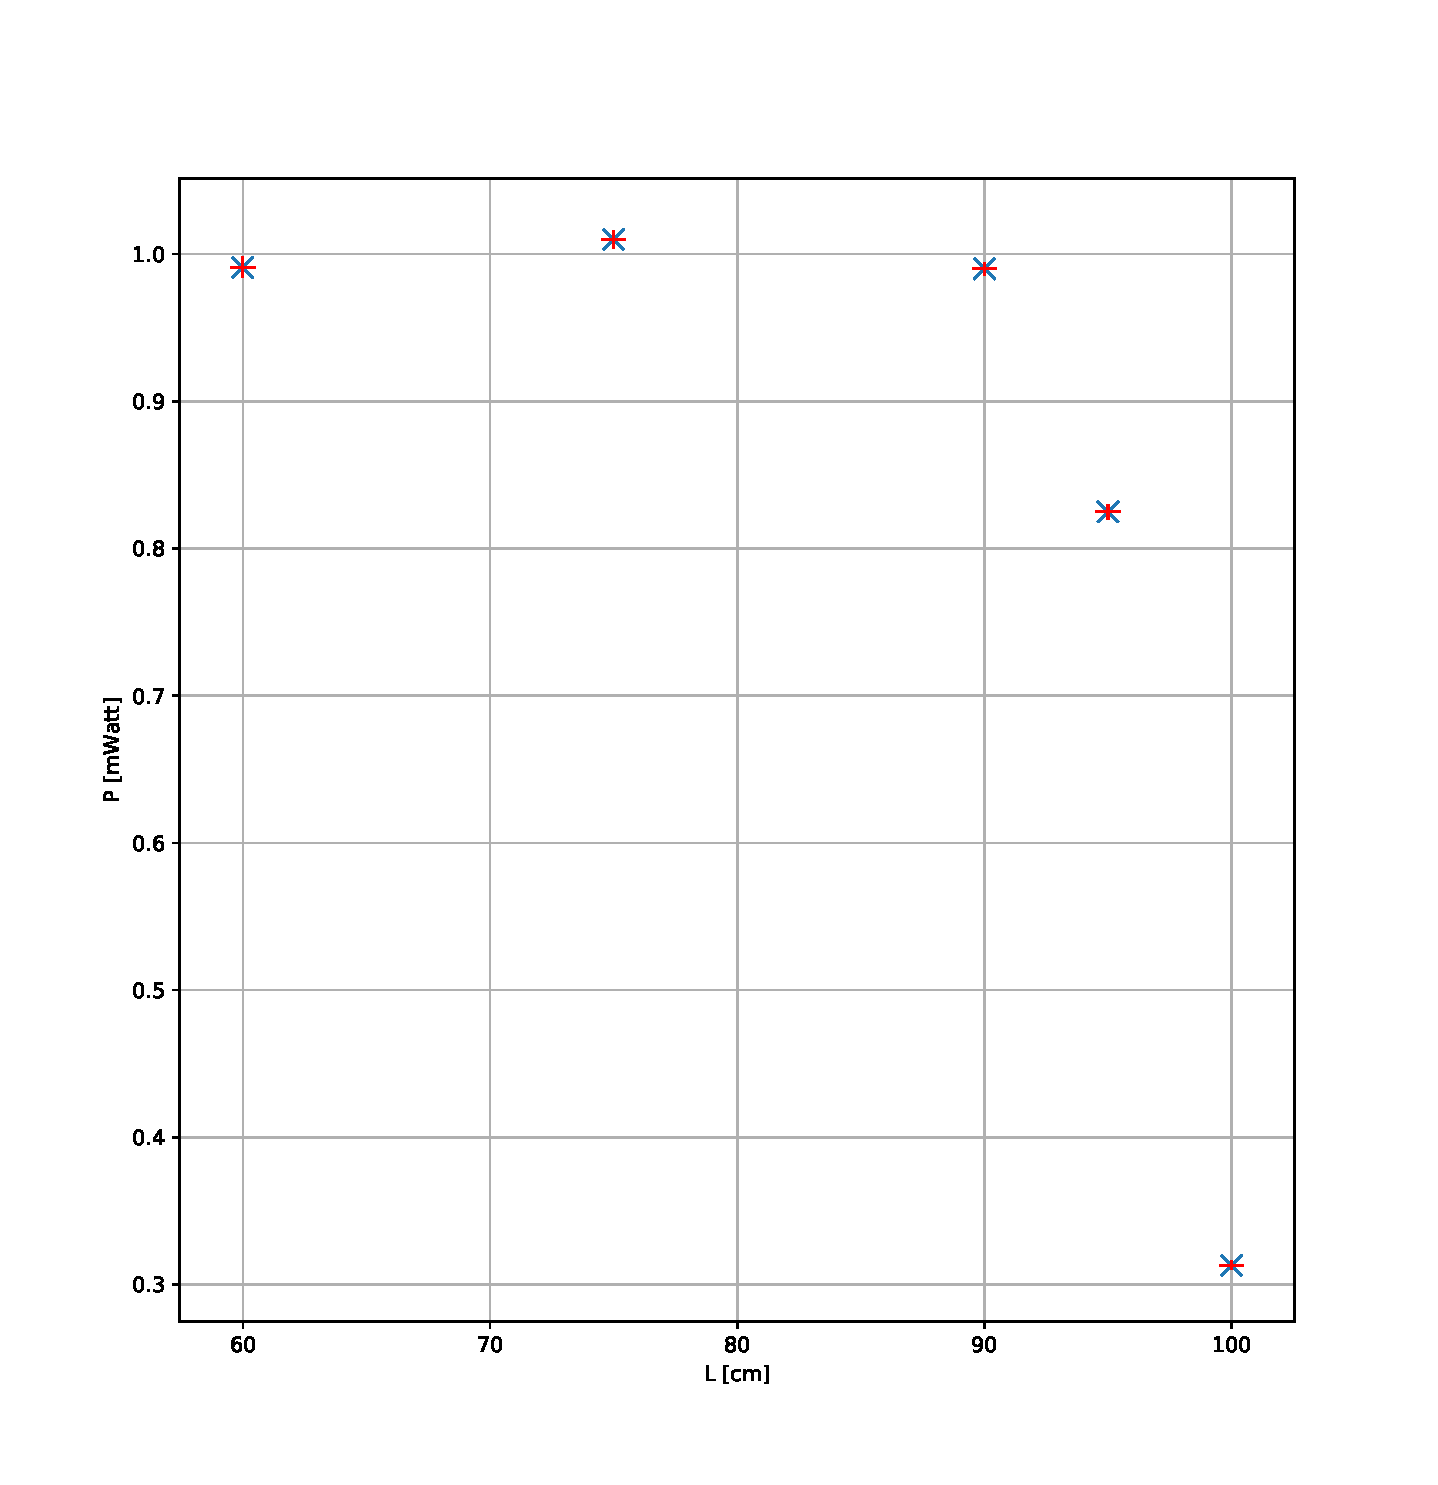
\includegraphics[width=.8\columnwidth]{figs/power-over-l.pdf}
  \caption{Maximale Durchschnittsleistung in Abh\"angigkeit der Resonatorl\"ange }
  \label{fig:power-over-l}
\end{figure}

\begin{table}[h]
  \centering
  \begin{tabular}{SSS}
    \toprule
    {L [\si{\centi\metre}]} & {P [\si{\milli\watt}]} & {\(\Delta\)P [\si{\micro\watt}]}\\
    \midrule
    60  & 0.991 & 7.1  \\
    75  & 1.01  & 6.3  \\
    90  & 0.99  & 4.6  \\
    95  & 0.825 & 3.0  \\
    100 & 0.313 & 5.0  \\
    \bottomrule
  \end{tabular}
  \caption{Maximallestung in Abh\"angigkeit der Resonatorl\"ange }
  \label{tab:leistunglaenge}
\end{table}






\subsection{Polarisationseigenschaften des Laserstrahls}
\label{sec:diskpol}

Die im Laser verbauten Brewsterfenster erlaubten nur Moden mit einer
Polarisationsrichtung. Somit folgt die Transmission, wie
in~\ref{fig:malus} zu erkennen, sehr gut dem Gesetz von Malus.

Am der letzte Messwert liegt deutlich \"uber der theoretischen
Kurve und auch andere Punkte liegen neben der Kurve. Gr\"unde daf\"ur
k\"onnten ungenaue Einstellung und besondere Eigenschaften des Strahls
oder Filters sein.

\begin{figure}[H]\centering
  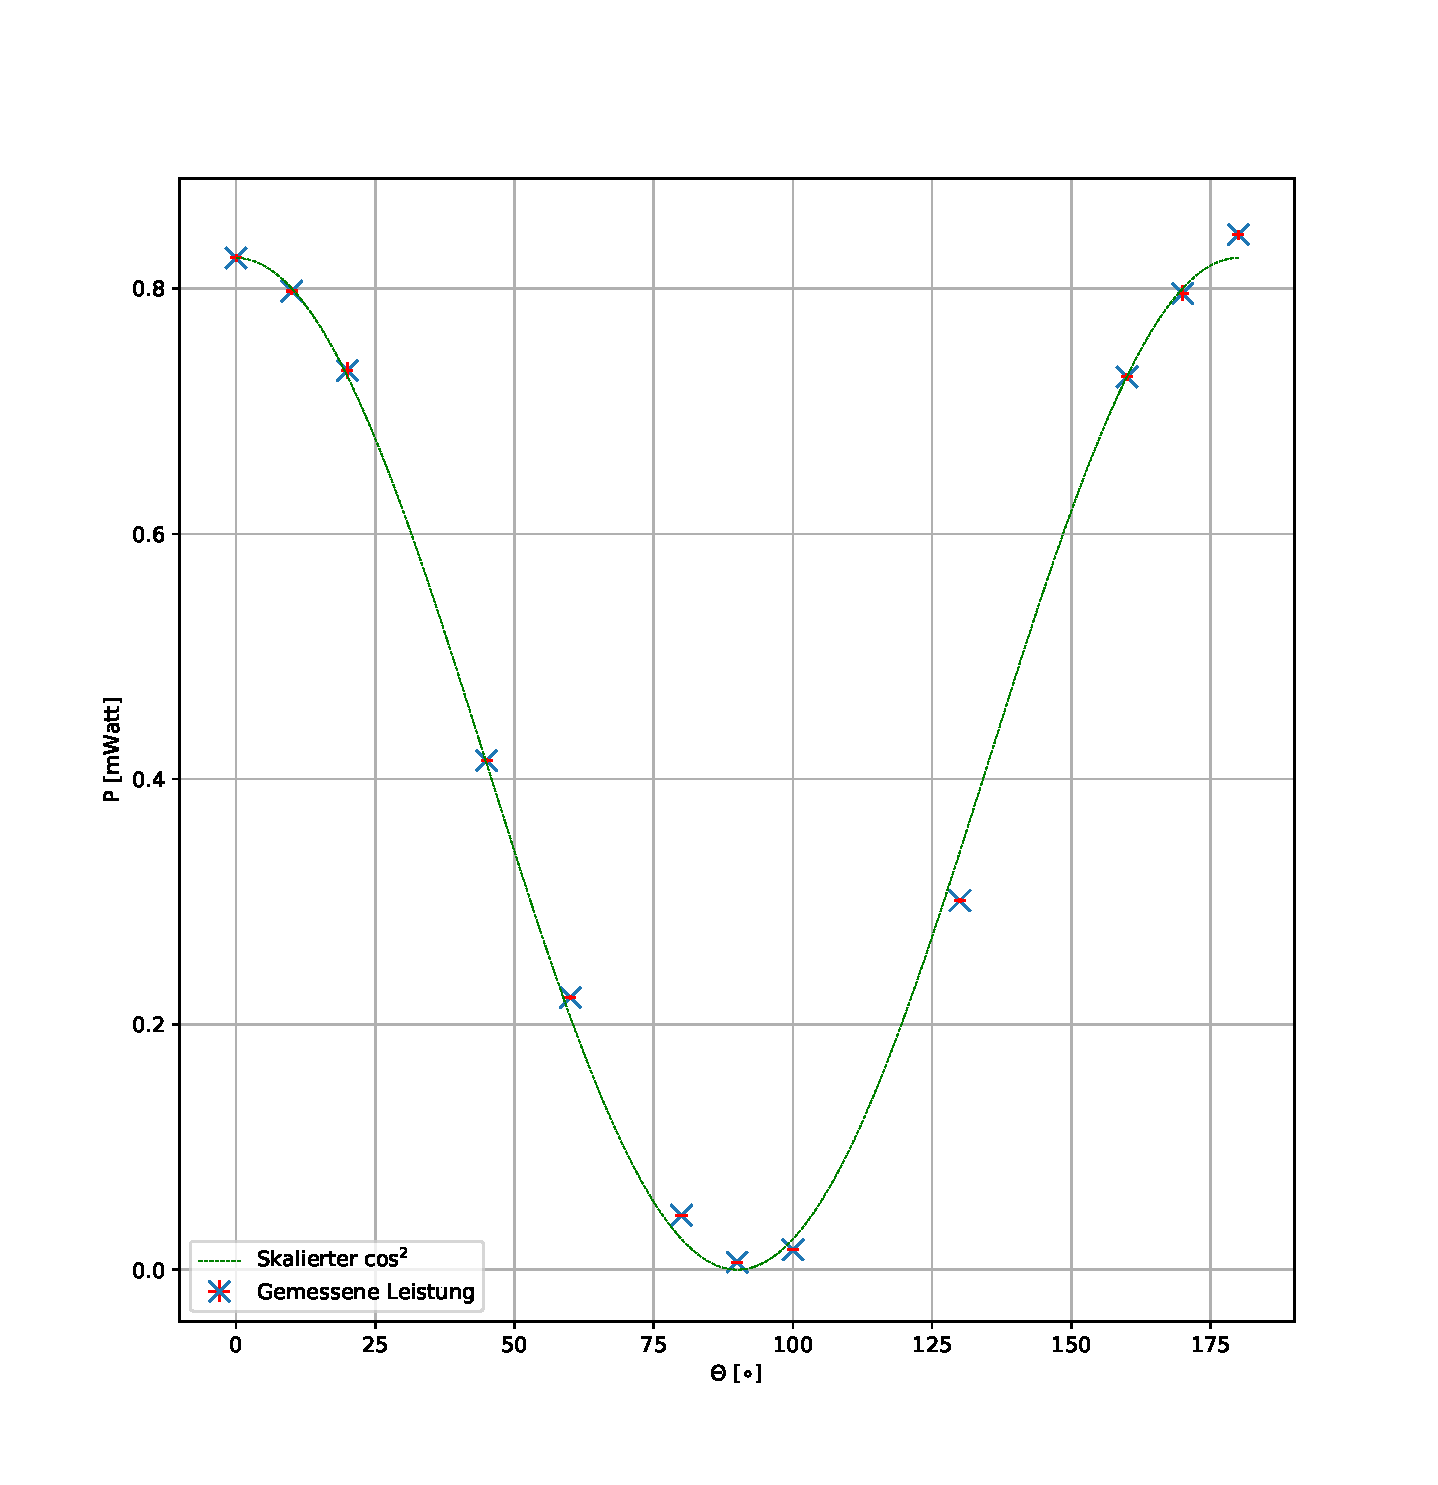
\includegraphics[width=.8\columnwidth]{figs/malus.pdf}
  \caption{Maximale Durchschnittsleistung in Abh\"angigkeit des Polarisationswinkels}
  \label{fig:malus}
\end{figure}

\begin{table}[h]
  \centering
  \begin{tabular}{SSS}
    \toprule
    {\(\Theta\) [\si{\deg}]} & {P [\si{\milli\watt}]} & {\(\Delta\)P [\si{\micro\watt}]}\\
    \midrule
    180 & 0.844   & 3.6     \\
    170 & 0.796   & 6.1     \\
    160 & 0.728   & 3.0     \\
    130 & 0.301   & 1.5     \\
    100 & 0.0163  & 0.084   \\
    90  & 0.00611 & 0.0066  \\
    80  & 0.0445  & 0.22    \\
    60  & 0.222   & 1.7     \\
    45  & 0.415   & 2.2     \\
    20  & 0.733   & 6.7     \\
    10  & 0.798   & 2.7     \\
    0   & 0.825   & 3.1     \\
    \bottomrule
  \end{tabular}
  \caption{Maximale Durchschnittsleistung in Abh\"angigkeit des Polarisationswinkels}
  \label{tab:malus}
\end{table}















\end{document}
